\chapter{Introduction}
Deep Neural Models have established themselves as standard-de-facto technology in most computer vision applications. This is due to the exceptional performances and versatile applicability they demonstrated in the last years. 
However, recent studies demonstrated that these models are susceptible to adversarial examples raising serious doubts on their reliability and trustworthiness, especially when embedded in real world safety and security-critical systems \cite{Szegedy2014IntriguingPO,Goodfellow2015ExplainingAH,Papernot2016TheLO, kurakin2016adversarial} .

Among these researches, the most studied scenario is image classification where the main adversarial objective is to cause system  misclassifications of data by applying some imperceptible image modifications.
In the last years several techniques for adversarial attacks have been proposed in literature. Most of them are settled in the white-box setting where it is assumed that the attacker knows details over the network structure or has access to the gradient values. It is clear that the applicability of such systems is relative low since any attacker cannot assume to have the necessary information \cite{Goodfellow2015ExplainingAH, madry2017towards, kurakin2016adversarial, carlini2017towards,Papernot2016TheLO}.

If we are looking for techniques with a concrete real-world applicability we have to move to the black-box setting. In this case the performance clearly decreases: the attack success rates are in general lower and the modifications applied to the images more visible. Interesting works are the ones proposing unrestricted attacks where the image modifications are not $L_p$-norm bounded: they employ large and visible perturbations while keeping the images realistic, natural looking and non-suspicious. The idea is to obtain images that can admit great differences from the original ones but, without a direct comparison with the original image, they cannot be distinguished from any other real (maybe filtered or edited) image. In this case the objective is not to limit the modifications on pixels but to limit the human perception that a modification has been applied \cite{Colorfool,ACE,wang2021demiguise}.

Extensive efforts have been made to combat these adversarial attacks. Some of them try to find noise, injected patterns and irregularities in the high frequencies image \cite{moosavi2018divide,liao2018defense}, while others try to build robust models adversarially trained \cite{andriushchenko2020understanding,bai2021recent}. 

The problem of achieving realistic attacks and effective defenses becomes more interesting and challenging for more difficult visual recognition tasks including object detection, especially due to their wide applicability to a lot of real-world critical systems such as autonomous driving \cite{feng2021review}, medical imaging \cite{chen2022recent} and smart cities \cite{ahmed2021adapting}. For these tasks,
the number of targets that need to be attacked is much larger
than that in pure classification task \cite{bose2018adversarial}. Moreover, in the case of models implementing the non-maximum suppression module (NMS),  even if a bounding box is successfully attacked, another sub-optimal bounding box may be detected in similar locations. As a matter of fact, it has been shown that existing attack methods primarily designed for classification do not generalize well to object detection \cite{shen2019advspade}. 

Some attack and defense techniques have been introduced in literature but the topic remains largely unexplored, especially in the black-box scenario when only the predicted bounding boxes are accessible to the attacker. Adversarial attacks for object detection were systematically studied for the first time in \cite{xie2017adversarial}.
Then, other approaches have been proposed \cite{arnab2018robustness,liang2021parallel,wang2020adversarial,procNoise_co2019, gu2021adversarial, Lu_2020_CVPR}.  

Another aspect that has not been adequately addressed for object detection is the use of adversarial machine learning techniques as defense methods against private information extraction, especially from images posted on social networks. It has been shown that information can be easily extracted from dataset and learned model in the case of classification \cite{bae2018security,shokri2015privacy,mireshghallah2020privacy,AGV-wiiat}.
In this case having good images without artifacts, patches, or visible noise patterns becomes of primary attention. The use of attacking methods producing good-looking images able to inactivate the information extraction procedures heavily applied on the Web could be of interest for the whole society.\\

In this thesis we propose a new attack method for object detection where the attacks are performed by applying a composition of Instagram-style filters to the image. They are obtained using customized versions of AGV algorithm with multi-objective optimization \cite{agv1} \cite{agv2}. AGV is based on a nested evolutionary optimization technique that can be adapted to several problems acting on the definition of fitness function and targets to optimize. \\
We demonstrate how the AGV evolutionary approach is able to find effective attacks that can overcome the existing ones both in terms of precision and image quality. The main contribution of this thesis can be summarized in: (1) a new method to attack object detection systems producing natural images that can be used also as protection method against unauthorized information extraction on the Web (2) evaluation of the efficiency of our attacks to different object detection models (3) analysis of robustness of two of the most known models (DETR \cite{detr_paper} and different versions YOLO \cite{yolov3, yolov4}). 



\chapter{Background} \label{sec:background}

\section{Adversarial Attacks}
Adversarial attacks are methods to generate adversarial examples that should resemble a valid input for humans but cause a machine learning model to make mistakes.
Their main application is in the field of Computer Vision and in particular image classification, but their applicability has been demonstrated also in other fields. %{\bf[CITARE]}. 

Adversarial attacks can be characterized in several ways. The main one considers the knowledge of the attacker about the victim. \textit{White-box} attacks work by having full access to the model and all its parameters and training details. This was the first case of study, but clearly the assumptions made are too strong to be applied for real-world attacks. 
%%cito esempi attacchi whitebox
\textit{Black-box} attacks, on the other hand, do not have full access to the model and nor to its internal structure.
They only have access to the output for a given input sample.
%%cito esempi di tipi di attacchi blackbox che utilizzando diversi approcci con pro e contro

Moreover, attacks can be classified as {\it restricted} or {\it unrestricted}, considering the amount of modifications they apply to the images in order to fool the systems. 
Restricted attacks generally use a $L_p$-norm distance to bound the modifications. The attacks are crafted with the aim of minimizing the differences between the original image and the adversarial one, even if it means having visible (more or less) artifacts. %In Figures \ref{fig:restricted_tifsgm_adv} and \ref{fig:restricted_sgm_adv}, the attacks produced by \cite{translation_invariant} and \cite{skip-matter}, two of the most recent state-of-the-art adversarial methods, are shown. In both the cases the generated artifacts are clearly visible. \\ 
%\item
Unrestricted attacks use large and visible perturbations while keeping the images realistic, natural looking and non-suspicious. The idea is to obtain images that can admit great differences from the original one but, beyond a direct comparison between the two, they cannot be distinguished from any other real (maybe filtered) image. %In Figures \ref{fig:unrestriced_ace_adv} and \ref{fig:unrestricted_colorfool_adv}, the attacks produced by ACE-Ins \citep{ACE_journal} and Colorfool \citep{Colorfool} are shown. 
The differences between the original image and the adversarial one are in general evident but, looking just at the adversarial one we might not be able to say that it is an attacking image.  
%\end{description}
 
Another aspect that has to be taken into account 
for real-world attacks is the amount of queries to the victim model that are necessary to craft effective attacks. Black-box systems, in general, need a huge amount of queries and, also in the case of systems built to work with limited access to the victim model, several thousands of queries are needed to produce reliable attacks.

\section{Object Detection}
%\subsubsection{Object Detection} 
\textbf{Object Detection} is the task of detecting objects in an image and assign them a label from a certain class. In its general formulation the aim is both to locate and classify multiple objects in a given scene.

Formally, given an object detection model $F$, $x \in \mathbb{R}^{(H \times W \times 3)}$ a 3-channel RGB image $x$ with height $H$ and width $W$ and a list of predefined classes $C$, the object detection output is a list of $M$ objects, each characterized by a rectangular bounding box of vertices $b_i=((x_{0i},y_{0i}),(x_{1i},y_{1i}))$ and a class label $c_i\in C$ as shown, for example, in Fig.\ref{fig:objdet_samples}.


% $F(x) \in \mathbb{R}^{M\times (4+1)}$ s.t. $F(x)=\{(b_i,c_i), i=1,...,M \}$, where $b_i \in \mathbb{R}^4$ is the bounding box for object $i$, $c_i\in C$ is its class label and $M$ is the number of the identified objects.\\


%\subsubsection{Adversarial example on object detection}
\textbf{An adversarial example against object detection}  is an image $x^*$, a modified version of $x$, such that, at least one object (possibly all the objects) recognized in $x$ is not identified or correctly classified in $x^*$. 
This means that $\exists i=1,...,M$, such that either $\nexists j=1,...,M^*\quad  s.t. \quad IoU(b^*_j,b_i) > threshold$ or $ c^*_k\neq c_i \quad \forall k=1,...,M^*\quad  s.t. \quad IoU(b^*_k,b_i) > threshold$, where $IoU(b_j,b_i)$ is the usual \textit{Intersection Over Union} measure used in computer vision between two generic bounding boxes $b_i$ and $b_j$.

% recognized  given  $F(x^*)=\{(b_i^*,c_i^*), i=1,...,M^* \}$
% \begin{equation} \label{eq:advDef_objdet}
%  \quad IoU(b_i^*,b_i) < threshold \qquad \vee \qquad  c_i^*\neq c_i,    
% \end{equation}
% for at least one, but possibly for all, object  
% For each object in the image $x$ the \textit{Intersection over Union} (IoU) between the new bounding box and the original one is under a given threshold or the classification label is different.

\subsection{State-of-the-art models}
The state-of-the-art methods for object detection can be categorized in one-stage and two-stage methods.
One-stage methods only need to go through the network once to locate objects and get their class. The most representative models are YOLO \cite{yolov3,yolov4}, RetinaNet \cite{retinanet}, SSD \cite{ssd} and DETR \cite{detr_paper}.
Two-stage methods treat object detection as a two stage problem: the first stage generates region proposals, including the object's approximate location, while the second classifies and precisely locates the object inside the proposed region. Some of the most famous and best performing two-stage object detectors are Faster R-CNN and Mask R-CNN.



\subsection{YOLO}
 
In this thesis we focus on attacking object detection systems based on YOLO (You Only Look Once) which is a state-of-the-art object detector with real time detection capabilities and high accuracy. 

%“You Only Look Once” YOLO Invented by Joseph Redmon, Santosh Divvala, Ross Girshick, and Ali Farhadi (2015) 
The first version of Yolo was introduced in \cite{redmon2016you} as a model that reframes object detection as a single regression problem to spatially separated bounding boxes and associated class probabilities. 
Over the years different YOLO versions have been released and nowadays YOLOv3 and YOLOv4 are among the most powerful and used models.

\textbf{YOLOv3} uses Darknet-53 to perform feature extraction, %this network as the name suggests ii is composed of 53 convolutional layers with shortcut connections.
a convolutional neural network composed of 53 convolutional layers with shorcut connections.
%\cite{yolov3}
The YOLOv3 algorithm first separates an image into a grid. 
Each grid cell predicts some number of anchor boxes around objects that score highly with the set of predefined classes.
This procedure can result in several overlapping bounding-boxes that are later corrected using Non-Max Suppression (NMS).
NMS is performed selecting the box with the highest score, calculating the interval overlap of this box with other boxes and omitting the boxes that overlap significantly.
To know which boxes overlap significantly it uses the measure of IOU (Intersection over Union): the greater the region of overlap, the greater the IOU.

\textbf{YOLOv4} is an improvement of the Yolov3 algorithm obtained by expanding the  Bag-of-Freebies (BoF) feature list that increases the detector accuracy without affecting the speed, like for example the use of genetic algorithms for
selecting the optimal hyperparameters, the use class label smoothing for sigmoid activation and the use of Cross mini-Batch Normalization, and many others. Authors showed to reach a mAP increment of 10\% increasing the processed  frames per second (FPS) by 12\%.

\subsection{DETR}
\textbf{DETR} (\textbf{DE}tection \textbf{TR}ansformer) is a new technique introduced by the Facebook research team in an article titled "End-to-End Object Detection with Transformers", presented in 2020 \cite{detr_paper}.
It’s a new object detection model created using Transformers architectures generally used in NLP.\\

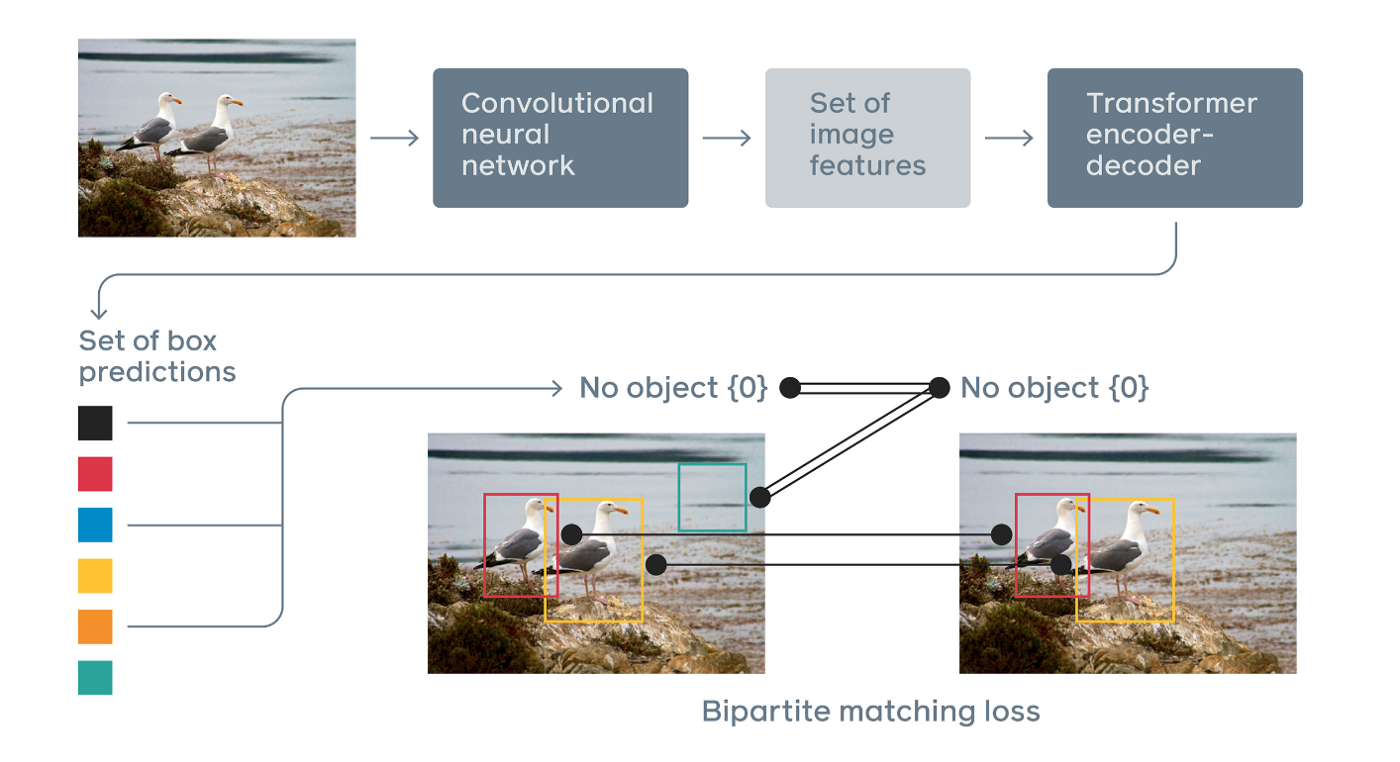
\includegraphics[width=\textwidth]{Introduzione/imgs/detr_architecture.png}\label{fig:detr_architecture}
As shown in (fig: \ref{fig:detr_architecture}) DETR directly predicts (in parallel) the final set of predictions by combining
a CNN with a transformer architecture. \\During training, bipartite matching
uniquely assigns predictions with ground truth boxes. Prediction with no match should
return a "no object" class prediction \cite{detr_paper}.


DETR is fast thanks to this parallel processing capability and for the fact that it doesn't use restrictive techniques such as anchor boxes and NMS, but it requires a lot of gpu memory compared to the other tested models.

It reaches very good performance, both in terms of  accuracy and run-time, very similar to the well-established and highly-optimized Faster RCNN baseline on the COCO dataset.
DETR achieves 42.0 AP computed on COCO 2017 val5k, with 0.036s inference time evaluated over the first 100 val5k COCO images.